\documentclass{article}

\usepackage{graphicx}
\usepackage{blindtext}
\usepackage{subcaption}
\usepackage{titling}
\usepackage{hyperref}
\usepackage[a4paper, total={6in, 8in}]{geometry} 


\pretitle{
  \begin{center}\LARGE
}

\posttitle{
  \\[0.5ex]
  \rule{\textwidth}{0.8pt}
  \vspace{1ex}
  \end{center}
}

\title{ECE 285 Final Project Proposal \textendash \@ Autonomous Vehicle Decision Making Through GAN's} 

\author{
  Anton John Del Mar \\
  Electrical and Computer Engineering \\
  A16728417 \\
  \and
  Daniel Chen \\
  Electrical and Computer Engineering \\
  A17061131 \\
}

\date{April 27, 2025}

\setlength{\droptitle}{-4cm} 

\begin{document}

\maketitle

\begin{abstract} 
    In our project¸ we aim to create a Conditional DCGAN to generate traffic signs that will be used to help train a traffic sign detection model for an autonomous vehicle (AV). We hope to create a generative model that can generate synthetic images to train the detection model and yield an accuracy close to a detection model trained on real images. This project will serve to show the usefulness of generative models in the evergrowing robotics world while also providing a practical model for AV's. 
\end{abstract}

\begin{figure}[h]
    \centering
    \begin{subfigure}{0.4\textwidth}
        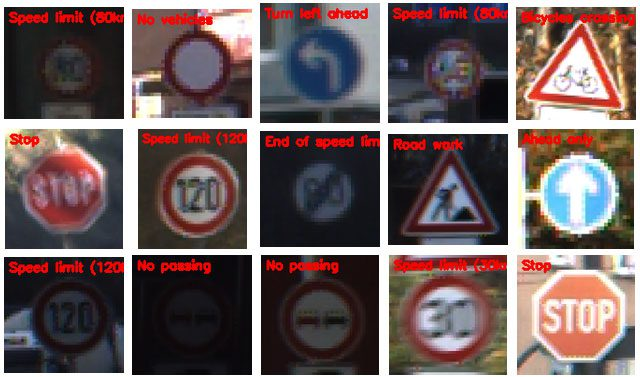
\includegraphics[width=\linewidth]{Pictures/traffic_sign_recognition_featured.jpg}
        \caption{Cropped Traffic Sign Images}
    \end{subfigure}
\end{figure}

\section{Motivation}
\qquad We were motivated to pursue this project because after taking ECE 148, an Autonomous Vehicle course at UCSD, in which we created a self-driving RC car, we noticed that one of the limitations of training a model for our vehicle was a lack of data. For example, on Kaggle there are mostly European based traffic sign datasets. We want to see if we can address this lack of data by testing the viability of realistic generated images in training street sign recognition. If proven viable, this could help accelerate AV training.

\section{Problem Definition}

\qquad With the use of a generative model we hope to resolve the issue of not having enough data. In Dewi’s paper \textit{Yolo V4 for Advanced Traffic Sign Recognition With Synthetic Training Data Generated by Various GAN} \hyperref[Dewi]{[2]}, they test various GAN's to generate synthetic images to expand their dataset, ultimately training a YoloV4 model with a dataset comprised of both synthetic and real images. Using DCGAN to generate a mixed training set allowed their YoloV4 model to achieve \%82.5 accuracy, when detecting traffic signs on a test set. Based on the results of Dewi’s paper we see that using generated images mixed with real images for a classification model gives useful results. Our aim of the project however is to test and see if synthetic images are viable as their own dataset, so we will create one set with only synthetic images and one set with only real images, and train two separate classification models to test classification accuracy on the same test set with new real images. We will keep in mind our own computational limitations since we have to run a simpler model given the course resources.

\qquad With the rapid progression of AV's, creating accurate sign and object detection models is essential for our safety. In the paper \textit{Traffic Signs Recognition using CNN and Keras in Python} \hyperref[Gupta]{[1]}, Shikha Gupta was able to make a traffic sign model that yielded an accuracy of around 95\% using CNN's on the German Traffic Sign Recognition Benchmark (GTSRB) dataset. \@ We will build off of Gupta’s CNN, improving the structure and tuning hyperparameters, in order to test if CNN models trained on our generated images can be as accurate of a classifier as the same CNN model trained on real images.


\begin{figure}[h]
    \centering
    \begin{subfigure}{0.8\textwidth}
        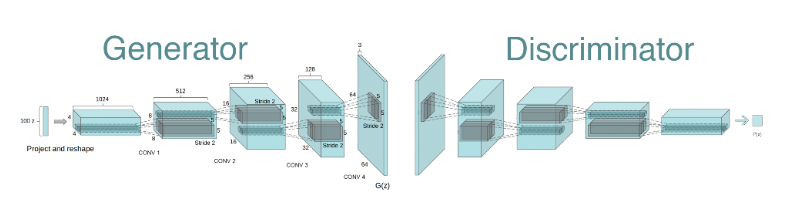
\includegraphics[width=\linewidth]{Pictures/DCGAN.png}
        \caption{DCGAN Structure}
    \end{subfigure}
\end{figure}

\section{Tentative Method}

\qquad For this project we will reimplement Gupta's base model \hyperref[Gupta]{[1]}which uses four convolutional layers, two max pooling layers, two dropout layers, two fully connected layers (one being the softmax layer), ReLU activation function, and finally an Adam optimizer. We plan to expand off this base model and add more blocks to the architecture that involve convolution, maxpool, and dropout layers in that order. We hope that the model we trained on the generated images can perform as well as the model trained on real images.

\qquad The Conditional DCGAN will be implemented using a basic architecture because Dewi’s paper \hyperref[Dewi]{[2]} does not mention the exact structure of their DCGAN. For our generator we will use convolutional transpose layers, batch normalization, and ReLU activation functions, where the input should be a latent vector drawn from a normal distribution and the output is an image. Then for the discriminator, we use strided convolutional layers, batch normalization, and leaky ReLU activation functions, where the output is the probability our input image is from the real data distribution or not. 

\qquad We choose a Conditional DCGAN because it excels in high resolution images while being relatively simple to implement as seen in Dewi’s paper. Our goal is to create new images for models to train on so real time generation/classification is not the priority. Therefore, it is worth the trade off of speed for high quality generated training images. 

\qquad The reason for choosing CNN’s is that they can yield high accuracy as seen in Gupta’s paper. Additionally, we are addressing the limitations of our resources because they are less computationally expensive to train compared to YOLO models, while still maintaining a high accuracy for a model trained specifically for traffic signs.

\section{Experiments}

\qquad We will be using the Laboratory for Intelligent and Safe Automobiles (LISA) dataset which is actually created by Prof Travaldi’s lab at UC San Diego \hyperref[LISA]{[5]}. It’s a well known dataset with a dash cam street view from across San Diego. However, there is no dataset widely available for cropped US street signs so we will use this dataset and crop the traffic sign images from it. From there we can use the cropped image dataset to train our generative street sign model to hopefully expand the existing street sign dataset for future AV sign recognition models to train on. 

\qquad In order to test the efficacy of this generated street sign image dataset, we will train two classifiers with the same algorithm, one entirely trained on real images and one entirely trained on our generated. Then we will have a single test set of real images that both models will be tested on. The difference in performance will tell us how well the generated images are for training compared to the real. If they are comparable in accuracy scores, then that means training on our generated image data set or at least augmenting existing real images with our generated image set would be helpful!

\qquad The data format for LISA is split by different driving scenes and lighting conditions. We will aim to be able to generate a diverse set of street signs under different lighting and weather conditions so having a dataset with diverse conditions to train on is essential. The dataset is one of the only US datasets and is perfect for our application. Many models are currently train on the German Traffic Sign Recognition Benchmark (GTSRB) \hyperref[GTSRB]{[3]} and Taiwan Road Marking Sign Dataset (TRMSD) \hyperref[TRMSD]{[4]}.

\qquad We can experiment with training on different sized cropped images from different size subsets of our LISA dataset. For example, we would test training on images 32x32 to 64x64 and likewise vary the generated output sizes to see performance and detection accuracy by our classifier.  We will also experiment with different GAN architectures, varying block organization and tuning hyperparameters. This will be a similar process to what we did in Homework 1 where we need to test many different permutations of our set of hyperparameters in order to train the optimal model performance for our application. 


\newpage

\begin{thebibliography}{9}

    \bibitem{Gupta}
    Shikha Gupta.
    \textit{Traffic Signs Recognition using CNN}.
    Analytics Vidhya, 2021.
    \url{https://www.analyticsvidhya.com/blog/2021/12/traffic-signs-recognition-using-cnn-and-keras-in-python/}
    
    \bibitem{Dewi}
    Ratna D. Dewi et al.
    \textit{Yolo V4 for Advanced Traffic Sign Recognition With Synthetic Training Data Generated by Various GANs}.
    IEEE, 2021.
    \url{https://ieeexplore.ieee.org/document/9471877}
    
    \bibitem{GTSRB}
    German Traffic Sign Recognition Benchmark (GTSRB).
    Kaggle Dataset.
    \url{https://www.kaggle.com/datasets/meowmeowmeowmeowmeow/gtsrb-german-traffic-sign}
    
    \bibitem{TSMRD}
    Taiwan Road Marking Sign Dataset (TRMSD).
    \url{https://www.researchgate.net/figure/Taiwan-Road-Markings-Sign-Dataset-TRMSD_tbl2_369461433}
    
    \bibitem{LISA}
    LISA Traffic Sign Dataset.
    UCSD Computer Vision and Robotics Research Lab.
    \url{https://cvrr.ucsd.edu/}
    
    \end{thebibliography}
    



\end{document} 